\chapter{Maze and Dungeon Generation}
Maze and dungeon generation has been around for some time but sadly still lacks significantly in the field of research. Basic maze generation algorithms already exist but only few attempts have been made to push these generic algorithms to the next level. Most maze generation algorithms are specialised graph-traversal algorithms that use pseudo-random number generators to visit cells of the dungeon in a random order. This chapter will discuss precisely how these various algorithms work, what features can be added to enhance them and how to apply these algorithms in a 3D application such as a video game. The aim of this chapter is to conceive a framework for procedural dungeon generation with maximum re-usability. Despite being targeted at dungeon-like environments, the features discussed in this section remains generic and can be used as a starting point for any 3D application that needs to make use of it.

\section{Maze Generation}
\subsection{Understanding Search-problems}
It has been observed that there are a large number of PCG techniques that are useful for a number of different kinds of environments. To generate a dungeon-like environment such as in the {\em Dungeons \& Dragons} pen-and-paper game a decision needs to made regarding what technique should be used to base the framework on. Judging by the results of mazes produced by Ashlock et al. it appears as though the search-based generation technique could be very viable \citep{DBLP:journals/tciaig/AshlockLM11}. In this the kind result that's desired and therefore the algorithms that will be discussed throughout this chapter will essentially be search-based.

Before going any further it is vital to understand exactly what is meant by a {\em search-based} algorithm. The idea behind a search-based algorithm is to start at a given state called the {\em start} state. From that initial state we can {\em transition} into a set of new  states and from those new state transition into even more states and so forth. The aim of these search-based algorithm is to try find a state that matches the {\em goal} \citep{DBLP:conf/cig/TogeliusPBWHY10}. Note that when that the structure of search problems can be viewed as traversing a graph: the states of the problem are the {\em nodes} in the graph and the transitions from one state to another are the {\em edges}.

\subsection{Properties of a maze}
Fortunately, mazes already have a rigorous and well-established mathematically model and theory that can be used to our advantage. We can define many properties for a maze but the most important ones in procedural dungeon generation are the following:
\paragraph{Unicursal} A unicursal maze is one with no junctions. Solutions of a unicursal maze are long winded paths \citep{ThinkLabyrinth}. 
\paragraph{Perfect} A maze can be considered as perfect if it has no cycles and no inaccessible areas \citep{ThinkLabyrinth}.
\paragraph{River} The term river is used to determine how much a maze ``flows". If the river factor is low then the maze will tend to have many short dead ends, otherwise if the river factor is high the maze will have fewer but longer dead-ends \citep{ThinkLabyrinth}.
\paragraph{Bias} Biased mazes will have passages that tend to favour a specific direction \citep{ThinkLabyrinth}. 

All the mazes that are generated by the framework are initially {\em perfect}, although that can be changed if required. Some algorithms will produce {\em biased} mazed, although most of them tend to produce un-biased mazes. The faster algorithms tend to be the ones that produced biased mazes \citep{ThinkLabyrinth}.

\subsection{Maze generation as a search-problem}
\subsubsection{The Graph}
As explained previously, a search-problem traverses various nodes and can visit adjacent nodes by using incident edges of the graph. The graph in this case can be viewed as a grid with cells.

\paragraph{Cells (nodes)} The cells in the grid represent a position $(x,\,z)$ in the maze. These cells correspond to the nodes of the graph. If a cell in the maze has at least one adjacent wall missing then it can be referred to as a {\em floor} cell, otherwise if the cell is completely walled off then it can be referred to as a {\em wall} itself or a {\em block}.

\paragraph{Walls (edges)} Each cell has a place on the top, bottom, left and right to position a wall. Each wall is shared between cells, and hence these walls correspond to the edges of the graph. The walls can either be {\em on} or {\em off} (no wall), although in practice this domain can be expanded to include objects such as doors for instance. Note that the walls on the very edge of the grid are only mapped to a single cell which doesn't make sense from a theoretical point of view. So in theory we can assume that the walls on the border are linked to cells are permanently inaccessible and invisible, although in practice those invisible cells can be ignored.

\begin{figure}[h!]
\centering
 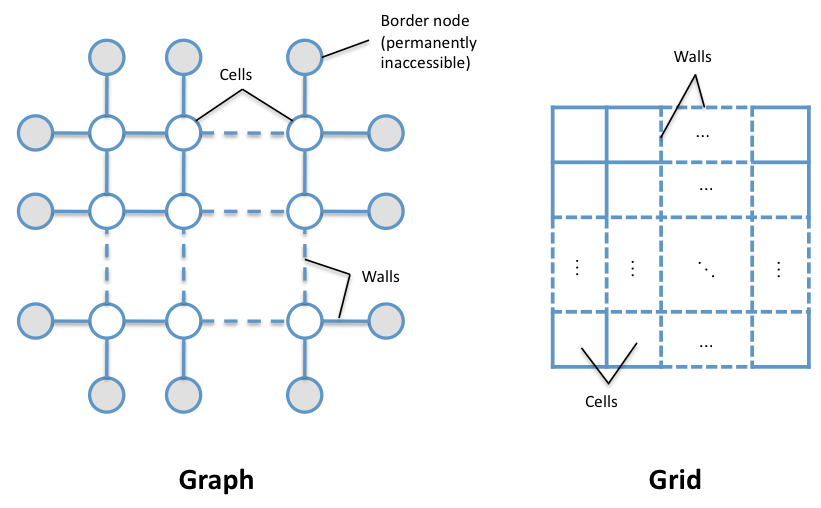
\includegraphics[width=0.87\textwidth]{images/graph-grid.png}
\caption{Graph and grid representations of the maze.}
\end{figure}

\subsubsection{The Goal}
In search problems the goal is a specific node that satisfies the desired conditions. Intuitively, one would believe that the start and end states of the search problem are the entrance (where the player starts) and the exit (where the player must get to) of the maze respectively. However, maze generators completely disregard the existence of such a concept. Instead, as explained by Pullen, all the maze generators will aim at generating perfect mazes and succeed to do so \citep{ThinkLabyrinth}. The two properties of a perfect maze, no cycles and no inaccessible cell, match exactly the definition of a {\em spanning tree\footnote{http://en.wikipedia.org/wiki/Spanning\_tree (Accessed on 15\textsuperscript{th} of July 2012)}} \citep{DBLP:journals/siamdm/Aldous90}. Therefore the goal of the search problem is to find a spanning tree.

\subsection{Depth-first search algorithm}
The depth-first search (DFS) algorithm is a simple way to implement maze generation. The classical depth-first search algorithm is modified slightly in this case to include the notion of random. Normally the children of a specific node are visited in an arbitrary order. However, in maze generation we will decide in which order the children should be visited at random. When visiting a new node the wall between the last visited cell and the new cell is removed. Upon reaching a node that has no un-visited children, we will backtrack and return to the last visited cell that still has unvisited children. The procedure is finished once there are no nodes to backtrack to (i.e. all the nodes have been visited).

Note that the DFS algorithm can be used for search-based algorithms. In this case however this is not the purpose of the DFS. We are simply using the DFS algorithm to create a random spanning tree. In other words, the DFS algorithm is only used to determine the transition from one state to another.

\lstAlgo
\begin{lstlisting}
Let M = the maze.
Mark each cell in M as "unvisited".
Let C = starting cell.
call DFS(C);

proc DFS(MazeCell C)
	while C has unvisited children do
		Pick random unvisited children D.
		Break walls between C and D.
		Mark D as "visited".
		call DFS(D);
	endwhile
endproc
\end{lstlisting}

We can observe that the depth-first search algorithm tends to provide mazes with a lot of very long paths (i.e. High river factor) \citep{ThinkLabyrinth}. This is because at the start of the algorithm very few cells are visited, hence the algorithm finds an unvisited child for each node more often than not, and hence backtracks very little. Therefore longer paths are generally caused because junctions are only created whilst backtracking which rarely occurs at the start. Later on, as the algorithm progresses, it finds more and more nodes with no unvisited children. So towards the end the algorithm tends to create more shorter paths and dead-ends become frequent.

\subsection{Prim's algorithm}
Another algorithm that is generally not used in search-problems is Prim's algorithm. Prim's algorithm is designed to find the {\em minimum spanning tree} of a {\em weighed undirected graph} using a {\em greedy method} \citep{Prim}. The idea behind the algorithm is to add the smallest weighed edge possible every iteration until all edges are included \citep{Prim}. The original algorithm is described below:

\lstAlgo
\begin{lstlisting}
proc Prim(Graph G)
	Mark each vertex in G as "unvisited".
	Let Es = All the edges of G.

	while (Total number of unvisited vertices) != 0 do
		Remove smallest weighed edged E from Es.
		Let C1, C2 = Vertices adjacent to E.
		
		if (E has at least 1 unvisited node) then
			Mark C1 and C2 as "visited".
			Add E to Es
		endif
	endwhile
	
	return Es // minimum spanning tree
endproc
\end{lstlisting}

Although Prim's original algorithm operates on the edges of the graph, it is possible to operate on adjacent nodes too \citep{DSAJ-4}. The modified version of Prim's algorithm for maze generation is expressed below:

\lstAlgo
\begin{lstlisting}
proc Prim(Maze M, MazeCell Start)
	Mark each cell in M as "unvisited".
	Let the set Cs = {Start}
	Mark Start as "visited".

	while Cs is not empty do
		Let C = random element of Cs.
		if (C has un-visited children) then	
			Let D = random un-visited child of C.
			Mark D as "visited".
			Break wall between C and D.
			Add D to Cs.
		else
			Remove C from Cs
		endif
	endwhile
endproc
\end{lstlisting}

Note that this modified version does not have the notion of {\em weight}. In the original algorithm we simply pick the edge with the smallest weight. However, in maze generation, we need to pick out a random edge from the set of available edges. From a conceptual point of view, the weights are assigned ``on the fly" and a random edge picked out as the minimum. 

Because of the nature of Prim's algorithm, the mazes constructed will look more ``spread out" than the depth-first search. In other words Prim's algorithm has the tendency to avoid creating very long paths \citep{ThinkLabyrinth}.

\subsection{Kruskal's algorithm}
Like the Prim's algorithm, Kruskal's algorithm is another greedy algorithm used to find the minimum spanning tree of a weighed undirected graph \citep{Kruskal}. The algorithm works by finding two unconnected trees in a {\em forest} and connecting them by removing the smallest weighed edge. The term {\em forest} refers to a set of trees that are not interconnected \citep{DSAJ-4}. The modified maze-generation version of the algorithm is given by:

\lstAlgo
\begin{lstlisting}
proc Kruskal(Maze M)
	Let F = Empty forest (set of trees).
	
	for each cell C in M
		Add the tree {C} to F.
	endfor
	
	for each wall W in M (in randomised order)
		Let C1, C2 be the two nodes connected by W.
	
		Let T1 = the tree in F that includes C1.
		Let T2 = the tree in F that includes C2.
		
		if T1 != T2 then
			Remove T1, T2 from F.
			Let G = T1 + T2 + W  // Connect T1 and T2.
			Add G to F.
		endif
	endfor
endproc
\end{lstlisting}

Because Kruskal's algorithm and Prim's algorithm both compute the minimum spanning tree they tend to provide mazes that look very similar to one another \citep{DSAJ-4}.

\subsection{Other algorithms}
Essentially, any algorithm that calculates a spanning tree of a graph can be used to generate a maze and several different algorithms exist \citep{AAJarai}. Other algorithms not based on spanning trees can also be used \citep{ThinkLabyrinth}. Pullen has enumerated the various different known algorithms that can be used in maze generation. However these other algorithms expose the inconvenience of being either slow or {\em biased} (meaning the maze has the tendency to follow a certain direction) \citep{ThinkLabyrinth}. 

\subsubsection{Aldous-Broder algorithm}
The Aldous-Broder algorithm got its name from its two creators: David Aldous and Andrei Broder \citep{DBLP:journals/siamdm/Aldous90}. The idea behind the algorithm is to generate a random {\em uniform spanning tree} as opposed to the minimum spanning tree from Prim and Kruskal's algorithms \citep{DBLP:conf/focs/Broder89}. A uniform spanning tree is defined as a spanning tree such that each edge has a uniform probability of getting picked\footnote{http://en.wikipedia.org/wiki/Uniform\_spanning\_tree (Accessed 16\textsuperscript{th} July 2012)}. The algorithm is expressed below:

\lstAlgo
\begin{lstlisting}
proc AldousBroder(Maze M, MazeCell Start)
	Initialize M such that all cells are "unvisited".
	Let C = Start.
	
	while M has unvisited cells do
		Let D = random neighbor of C.
		
		if D is unvisited then
			Mark D as "visited".
			Break wall between C and D.
			Let C = D.
		else if there is no wall between C and D then
			Let C = D.
		endif
	endfor
endproc
\end{lstlisting}

Because of the random nature of Aldous-Broder algorithm, it tends to produce mazes that are less biased and with a lower river factor than any other maze. However the algorithm is, on average, much slower than any other maze generation algorithms and isn't even guaranteed to terminate \citep{ThinkLabyrinth}.

\subsubsection{Wilson's algorithm}
This algorithm is an improved version of the Aldous-Broder algorithm and produces mazes that are the same \citep{ThinkLabyrinth}. However, Wilson's algorithm is much faster because it uses certain optimisation when retracing \citep{DBLP:conf/stoc/Wilson96}. On average, Wilson's algorithm is about 5 times faster than Aldous-Broder's algorithm, but 2 times slower than other algorithms \citep{ThinkLabyrinth}. 

\subsubsection{Hunt and Kill algorithm}
The Hunt and Kill algorithm is similar to the depth-first search algorithm; it differs only in the sense that it doesn't have backtracking. Instead, the algorithm starts in {\em Kill} mode and visits random cells breaking walls as it goes along just like the depth-first algorithm. However, once it reaches a dead-end it enters {\em Hunt} mode and scans the whole maze from top to bottom trying find an unvisited cell situated near a visited one; this substitutes the backtracking. It then breaks the wall between these two cells and returns to Kill mode. The algorithm is finished once the Hunt mode fails to find an unvisited cell \citep{ThinkLabyrinth}.

\subsubsection{Growing Tree algorithm}
The Growing Tree algorithm is very simple. It involves adding newly visited cells into a list and removing them once they have no more neighbouring unvisited cells. The algorithm simply picks a cell from this list and breaks a random wall. What's interesting about this algorithm is that is can provide entirely different results based on how elements are picked from the list. Example: picking the most recent cell causes the algorithm to behave exactly like the depth-first search algorithm \citep{ThinkLabyrinth}

\subsubsection{Eller's algorithm}
Eller's algorithm has the reputation of being the most memory efficient. It constructs the maze row by row and once a row has been constructed it is no longer referenced in the algorithm. As a direct result this means the entire maze does not always need to be in memory, only one row at a time is required. This property makes Eller's algorithm very convenient for large mazes \citep{ThinkLabyrinth}.

\subsubsection{Recursive Division algorithm}
This algorithm is very different to other algorithms because it does not explicitly refer to the cells in the maze. Instead, the algorithm simply recursively divides the maze into two sections and by adding a long vertical or horizontal wall and leaving gaps at random \citep{ThinkLabyrinth}.

\subsubsection{Binary Tree Mazes}
The Binary Tree algorithm is said to be the fastest maze generator possible, but unfortunately the mazes produced are very biased. The algorithm is as simple as: for each cell break either the left or upper wall. Since the cells are independent, the order in which the maze is traversed is irrelevant \citep{ThinkLabyrinth}.

\subsubsection{Sidewinder Mazes}
The sidewinder maze algorithm and binary tree algorithm are very similar although the sidewinder is slightly more complicated. The rows are constructed one at a time and all the passages of a sidewinder maze leading up will lead to the start of the maze. Solutions of sidewinder never visit a row more than once. Needless to say, the mazes created by the sidewinder algorithm are biased \citep{ThinkLabyrinth}.

\begin{figure}[h!]
\centering
 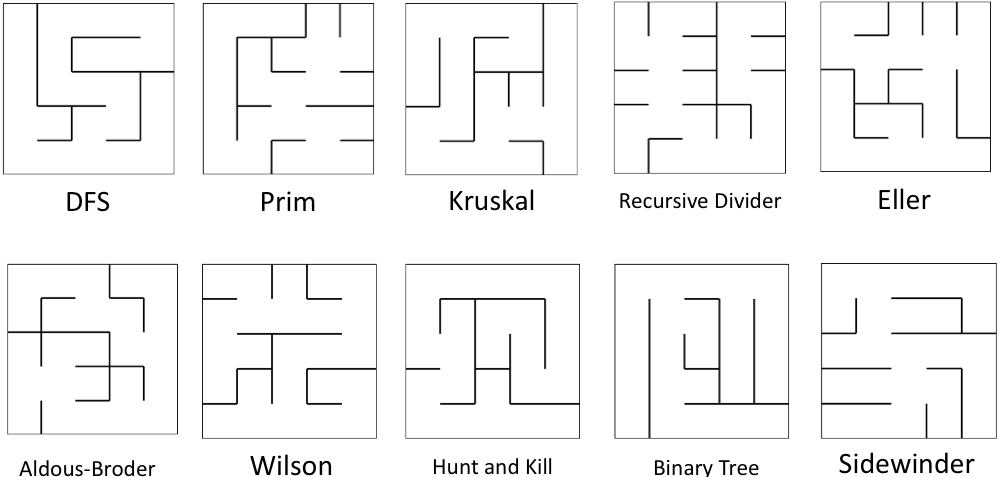
\includegraphics[width=1\textwidth]{images/mazes.png}
\caption{Sample mazes produced by different algorithms.}
\end{figure}


\section{Maze Post-processing}
So far only maze generation has been discussed, however this is not entirely the same as dungeon generation. The mazes that are generated by the maze algorithm have two properties that cause a problem:

\begin{itemize}
\item {\bf Density:} The mazes created are very dense. The term ``density" in a maze refers to the amount of cells that are accessible. In fact, the mazes produced are perfect and hence every cell is accessible from every other cell \citep{ThinkLabyrinth}. However according to Jamis Buck a dungeon will typically be very sparse and have many inaccessible cells \citep{JBuck}.
\item {\bf No loops:} Another property of perfect mazes is that they do not contain any loops \citep{ThinkLabyrinth}, although loops in a dungeon is considered normal \citep{JBuck}.
\end{itemize}

In order to transform the generated mazes into a dungeon-like environment these two properties must be obliterated through some post-process operations.

\subsection{Maze sparseness}
Making the maze more sparse is relatively simple. All that is needed to exclude certain cells from the maze, i.e. we need to wall off these cells completely. However we must insure that walling off a cell does not cause other accessible cells to become inaccessible. In others words, when we wall off a cell we should still end up with a single maze and not multiple independent mazes. Figure \ref{abcd-sparseness} shows an example of a bad implementation of sparseness: walling off cell B cause the cells A, C and D to become separate mazes. We want to insure that this doesn't happen. To avoid this we can simply specify the algorithm to wall off dead-ends only \citep{JBuck}, such as cells A, B or D in Figure \ref{abcd-sparseness}. It's trivial that walling off a dead-end only causes that cell to become inaccessible and doesn't affect any other cells.

\begin{figure}[h!]
\centering
 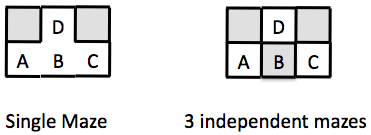
\includegraphics[width=0.38\textwidth]{images/abcd_sparseness.png}
\caption{An example of bad sparseness implementation.}
\label{abcd-sparseness}
\end{figure}

The {\em sparseness factor} defines how many iterations the algorithm should perform. The higher factor will naturally imply a sparser maze \citep{JBuck}. The implementation of this algorithm is expressed as the following (an example of this effect is show in Figure \ref{sparseness2}):

\lstAlgo
\begin{lstlisting}
proc DeadEndRemover(Maze M, Integer Sparseness)
	for I in [1, Sparseness] do
		for each cell C in M do
			if C is a dead-end then
				Wall-off C completely.
			endif
		endfor
	endfor
endproc
\end{lstlisting}

\begin{figure}[h!]
\centering
 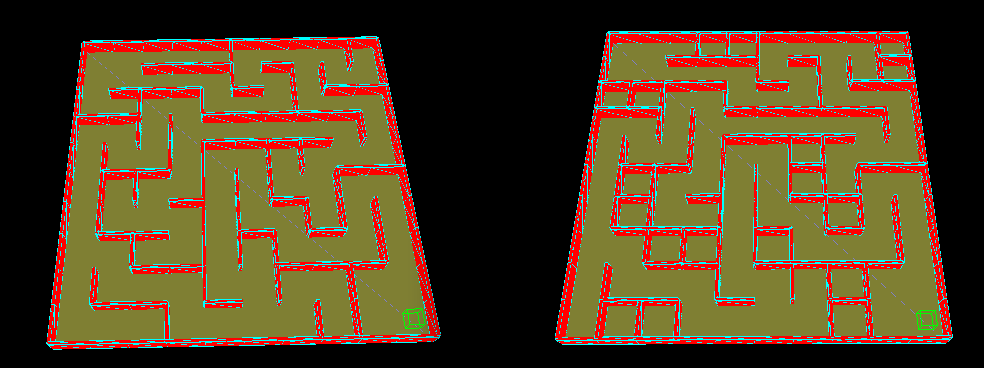
\includegraphics[width=0.74\textwidth]{images/DeadEndDigger-sparse2.png}
\caption{Effect of the dead-end remover with sparseness = 2.}
\label{sparseness2}
\end{figure}

\subsection{Adding loops}
Jamis Buck suggested a method to add loops which should be done after the density-reduction phase. The reason for this is that the concept behind this phase consists of ``restoring" some cells that have been excluded in the previous phase. To create a loop we simple take any remaining dead-end in the maze as a starting point. From this starting point perform a randomised search like with the DFS or Hunt and Kill algorithms. Once we reach a cell which is accessible, (i.e. it has at least 1 wall missing) we stop this search and repeat this process as many times as necessary. Because we break walls until we reach a cell that is part of the maze this causes a loop to be formed \citep{JBuck}.

\begin{figure}[h!]
\centering
 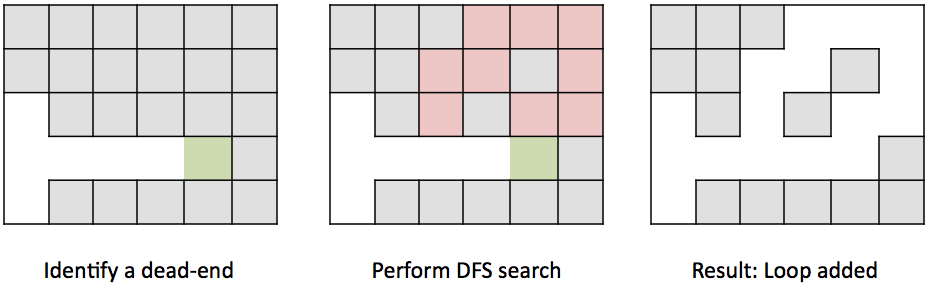
\includegraphics[width=0.74\textwidth]{images/adding_loops.png}
\caption{An example on how to add loops to a maze.}
\end{figure}

However Jamis Buck doesn't not appear to consider cases where the maze doesn't have any dead-ends, which can occur if the sparseness factor is too high. This scenario can be made less frequent by keeping the sparseness factor low but this does not guarantee the presence of dead-ends. There are two possible ways of enforce this phase:
\begin{enumerate}
\item {\bf Add dead-ends:} Before adding loops we could check to see if any dead-ends are present. If not, then we can add random uniformly distributed dead-ends across the maze.
\item {\bf Extending any cell:} We could also modify the original algorithm to start at any random accessible cell and not only dead-ends.
\end{enumerate}

Assuming that dead-ends are present, we can add loops using the following algorithm:
\lstAlgo
\begin{lstlisting}
proc AddLoops(Maze M, Integer NLoops)
	Let I = 0.
	while (I < NLoops) AND (M still has dead-ends) do
		Let C = Random dead-end.
		Let L = The cell that leads into C.
		while C is a dead-end do
			Let D = Step(C, L).
			Let L = C.
			Let C = D.
		endwhile
		Let I = I + 1.
	endwhile
endproc

func Step(Maze M, Cell C, Cell L)
	Let D = a random neighbouring cell of C other than L.
	Break walls between C and D.
	return D.
endfunc
\end{lstlisting}

\subsection{Adding rooms}
The dungeon will often have large rooms that the paths will lead to. Essentially adding rooms involves breaking all the walls in a certain area to open up a lot of space. The rooms themselves represent an empty rectangular area in the maze and can simply be defined by their width and length \citep{JBuck}. One naive approach to first create the dimensions of these rooms then position them anywhere in the maze using a uniform number generator:
\lstAlgo
\begin{lstlisting}
proc AddRooms(Maze M, Integer NRooms)
	for I in [1, NRooms] do
		Pick a random accessible cell C in M.  // use as the top-left
		Pick a random dimension [Width, Length].
		
		// Calculate bottom-right corners.
		Let A = M.GetCell(C.x + Width, C.z + Length).
		
		Break all the walls in between the cells C and A.
	endfor
endproc
\end{lstlisting}

This method is simple and very time efficient. It has a time complexity of $\bigo{n}$ where $n$ is the number of rooms added, which is convenient for very large mazes. However this method will not always give very convincing results because a room is meant to touch as few corridors and other rooms as possible \citep{JBuck}. Jamis Buck suggested a different approach where a {\em weighing system} is used. This consists of testing each possible position for a room and assigning a score to each position. The position with the lowest score is the considered the best solution \citep{JBuck}. The score for a given position and room is calculated using with algorithm:
\lstAlgo
\begin{lstlisting}
func CalcScore(Maze M, Cell Position, Integer RoomWidth, Integer RoomLength)
	Let X0 = Position.x
	Let Z0 = Position.z
	Let Score = 0.
	for I in [X0, RoomWidth] do
		for J in [Z0, RoomLength] do
			Let C = M.GetCell(Position.x + X0, Position.z + Z0)
			if (C is in index range) then
				for each corrider adjacent to C do
					Score = Score + 1.
				endfor
				if C is a corridor then
					Score = Score + 3.
				endif
				if a room is located at C then
					Score = Score + 100.
				endif
			endif
		endfor
	endfor
endfunc
\end{lstlisting}
This method will provide more decent results but it has to iterate over every cell in the maze to find the lowest score \citep{JBuck}. It has a complexity of $\bigo{nm^2}$ where $n$ is the number of rooms and $m$ is the dimension of the maze (assuming the dimension is square).

\begin{figure}[h!]
\centering
 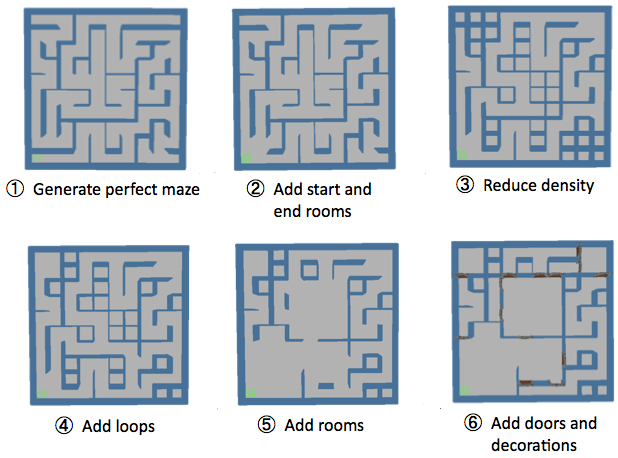
\includegraphics[width=0.8\textwidth]{images/phases-mixed.png}
\caption{The multiple different phases of the dungeon-generation algorithm.}
\end{figure}